\documentclass[paper=a4, fontsize=11pt]{scrartcl} % A4 paper and 11pt font size

\usepackage[T1]{fontenc} % Use 8-bit encoding that has 256 glyphs
\usepackage{fourier} % Use the Adobe Utopia font for the document - comment this line to return to the LaTeX default
\usepackage{amsmath,amsfonts,amsthm, amssymb} % Math packages
\usepackage{multirow}
\usepackage{hyperref}
\usepackage{sectsty} % Allows customizing section commands
\usepackage{graphicx}
\usepackage{tabularx}
\usepackage{enumitem}
\usepackage{wrapfig}
%---------
%CITATIONS
%---------
\usepackage[style=apa,backend=biber]{biblatex}
\usepackage{csquotes}
\usepackage[american]{babel} % English language/hyphenation
\DeclareLanguageMapping{american}{american-apa}
\addbibresource{sources.bib}

\usepackage{tikz}
\usepackage{calc}
\def\checkmark{\tikz\fill[scale=0.4] (0,.35) -- (.25,0) -- (1,.7) -- (.25,.15) -- cycle;} 
\def\scalecheck{\resizebox{\widthof{\checkmark}*\ratio{\widthof{x}}{\widthof{\normalsize x}}}{!}{\checkmark}}

\allsectionsfont{\centering \normalfont\scshape} % Make all sections centered, the default font and small caps

\usepackage{fancyhdr} % Custom headers and footers
\pagestyle{fancyplain} % Makes all pages in the document conform to the custom headers and footers
\fancyhead{} % No page header - if you want one, create it in the same way as the footers below
\fancyhead[L]{\tiny{\url{https://github.com/WhereIsJulius/AVC-Code}}}
\fancyhead[R]{\tiny{Jacob Beal\\300378461}}
\fancyfoot[L]{} % Empty left footer
\fancyfoot[C]{} % Empty center footer
\fancyfoot[R]{\thepage} % Page numbering for right footer
\renewcommand{\headrulewidth}{0pt} % Remove header underlines
\renewcommand{\footrulewidth}{0pt} % Remove footer underlines
\setlength{\headheight}{13.6pt} % Customize the height of the header

\numberwithin{equation}{section} % Number equations within sections (i.e. 1.1, 1.2, 2.1, 2.2 instead of 1, 2, 3, 4)
\numberwithin{figure}{section} % Number figures within sections (i.e. 1.1, 1.2, 2.1, 2.2 instead of 1, 2, 3, 4)
%\numberwithin{tabular}{section} % Number tables within sections (i.e. 1.1, 1.2, 2.1, 2.2 instead of 1, 2, 3, 4)

\setlength\parindent{0pt} % Removes all indentation from paragraphs - comment this line for an assignment with lots of text

%----------------------------------------------------------------------------------------
%	TITLE SECTION
%----------------------------------------------------------------------------------------

\newcommand{\horrule}[1]{\rule{\linewidth}{#1}} % Create horizontal rule command with 1 argument of height

\title{
\normalfont\normalsize
\textsc{Victoria University, ENGR101} \\ [25pt] % Your university, school and/or department name(s)
\horrule{0.5pt} \\[0.4cm] % Thin top horizontal rule
\huge AVC Project Report\\ % The assignment title
\horrule{2pt} \\[0.5cm] % Thick bottom horizontal rule
}

\author{Jacob Beal} % Your name

\date{\normalsize\today} % Today's date or a custom date
\begin{document}
\maketitle
\tableofcontents
\section{Abstract}
The Following Lab Report details how the application of fundamental engineering
concepts could be used in such a way to construct and operate an Autonomous
Vehicle. This report will detail the design, construction, and programming
decision that we made, the final outcome of the project and the end results,
and in particular issues that arose, and how this was resolved.\\

The Robot in question did not complete the entire maze, and did not complete the
Third Quadrant.
\section{Introduction}
\subsection{Motivation}
The purpose of the AVC is to demonstrate engineering skills taught in the
ENGR101 Labs; and to work as a team to create an autonomous vehicle. This is
used to solidify the teams understanding of fundamental Engineering concepts.
\subsection{Problem}
The challenge of a self-driving car is not immediately intuitive; the act of%TODO
simply ``following a line``. This involves computing the relative position of
the vehicle compared to the line. The team employed other methods, by tracking
the relative position over time, that will be detailed later in the report.
\subsection{Scope}
The scope of this project was using C/C++, the ENGR101 C Library and skills we
have learned in the Labs for the project. This includes \textit{PID} Error
Correction (Proportional, Integral and Derivative Responses) to follow the 
white line and other techniques taught in lectures.\\
We are also limited by our budget of $V\$100$ for use at the \textit{``part
  bazzar``} and the equipment that were provided at the beginning of the
project, the Roboshield, motors and Raspberry Pi.

\subsection{Motivation}
Understanding how an AVC works and solving a problem is important to the future,
with autonomous vehicles increasing in prevalence, and being developed at break
neck speed, it is of paramount importance that we understand how they work, and
their limitations.
\section{Background}
\subsection{Theory}
\subsubsection{Closed Loops}
A closed loop system is a system which constantly loops, checking a physical
variable. This variable is then computed in such a fashion as to deliver an
output which is used in such a method to influence the physical variable the
next time the loop is checked.\footcite{elfClosedLoops}

A closed loop system is useful in the ``follow the line'' section of the AVC
where a difference in position of the line and the centre of the camera, which
can be used to generate a difference in wheel speed. This difference in wheel
speed can cause a turn in the vehicle

\begin{figure}{h}
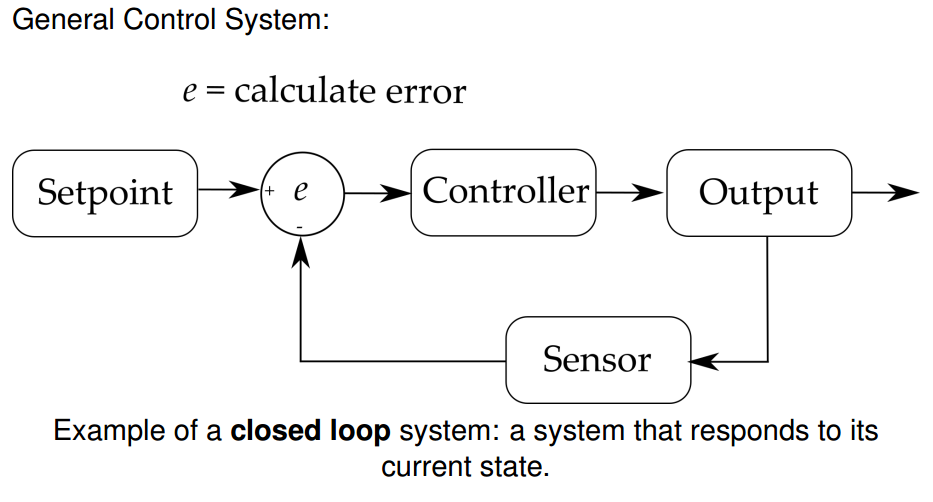
\includegraphics[width=\textwidth]{closedloop}
\centering
\caption{A Closed loop diagram \autocite{elfClosedLoops}}
\end{figure}

\subsubsection{PID}
\textit{PID} stands for \textit{Proportional, Integral and Derivative} response
to a change in the conditions in a closed loop.\\
A proportional response is the current conditions and how it responds to them
immediately.\ i.e.\ the further the object is from the line, the stronger
corrective response is.\\
A integral response checks over time to see whether the car is on one side too
often, and compensates accordingly.\\
A derivative response is related to how quickly the proportional response
changes, and therefore turns the car the other way when it approaches the line.
\begin{figure}[h]
  \centering
  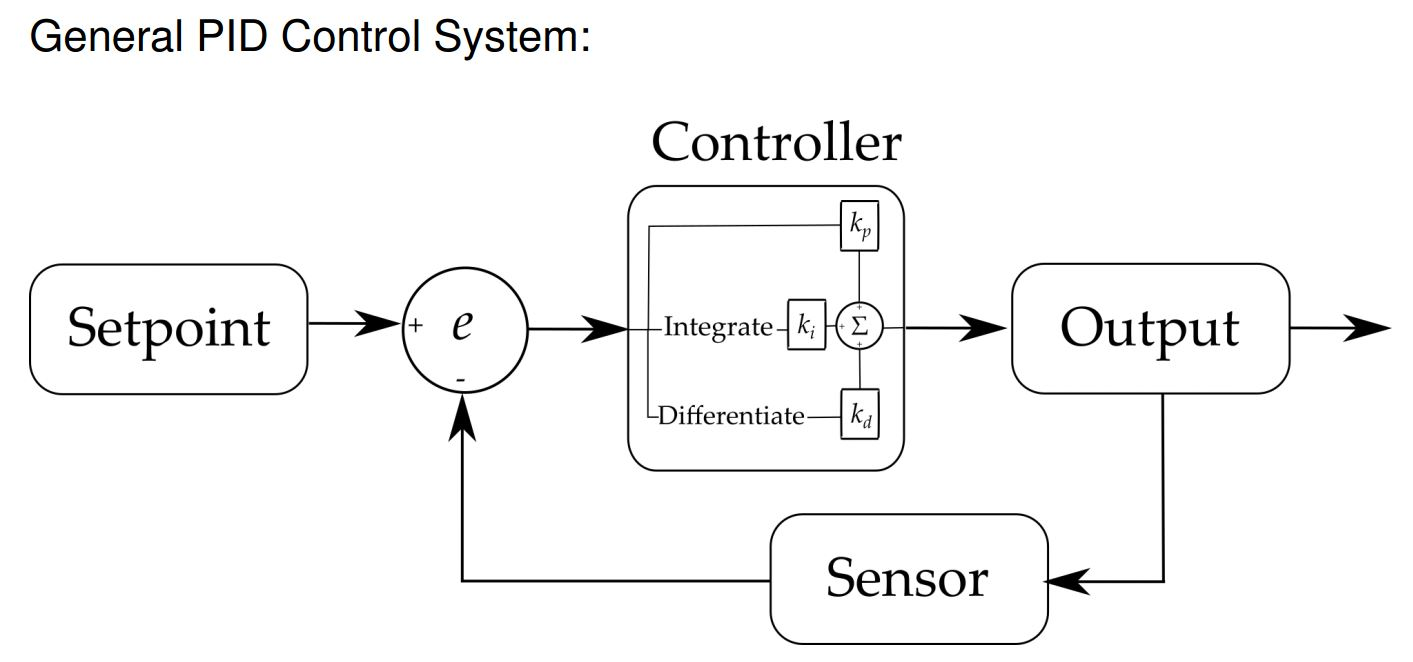
\includegraphics[width=\textwidth]{pid.png}
  \caption{A PID system diagram\autocite{elfClosedLoops}}
\end{figure}
\subsubsection{C and Raspberry Pi}
The project will be written using C++, with  an imported C library for the
functionality to control the motors and receive input from sensors.\\
\subsection{Research}
Tuning the PID system should be done in the specific order of Proportional,
Integral then derivative responses. This is because the integral response can
only be turned following the proportional response, so the offset at the end of
the sinusoidal activity, and the derivative response merely acts as a
dampener\footcite{pidTuning}
\footcite{pidVid}
\section{Methods}
\subsection{Equipment}
The AVC Project was based on a Raspberry Pi and the Roboshield.\\
The Autonomous vehicle was built with a `PiCam' camera (provided), a pair of
motors (provided), 2 `Sharp GP2Y0A41SK0F Analog Distance' sensors, a 3D printed
chassis, and half a ping pong ball.
\subsection{Procedure}
\begin{wrapfigure}{r}{0.5\textwidth}
  \begin{center}
    \includegraphics[width=0.3\textwidth]{top-down-diag}
    \caption{A top-down view of the design chosen for the AVC}
  \end{center}
\end{wrapfigure}
The team first designed the layout of the vehicle. The chosen design is based
primarily on the given initial board. From this the motors were mounted at the
front (See Fig 4.1), and the rear wheel, a semi-sphere, was chosen. A
semi-sphere was chosen so that it had no bias in direction, nor resistance to
change in direction, so that it could react better to change in direction.\\

\section{Results}
\subsection{Data}
The gate at the beginning now opens on request.
\begin{figure}[h]
  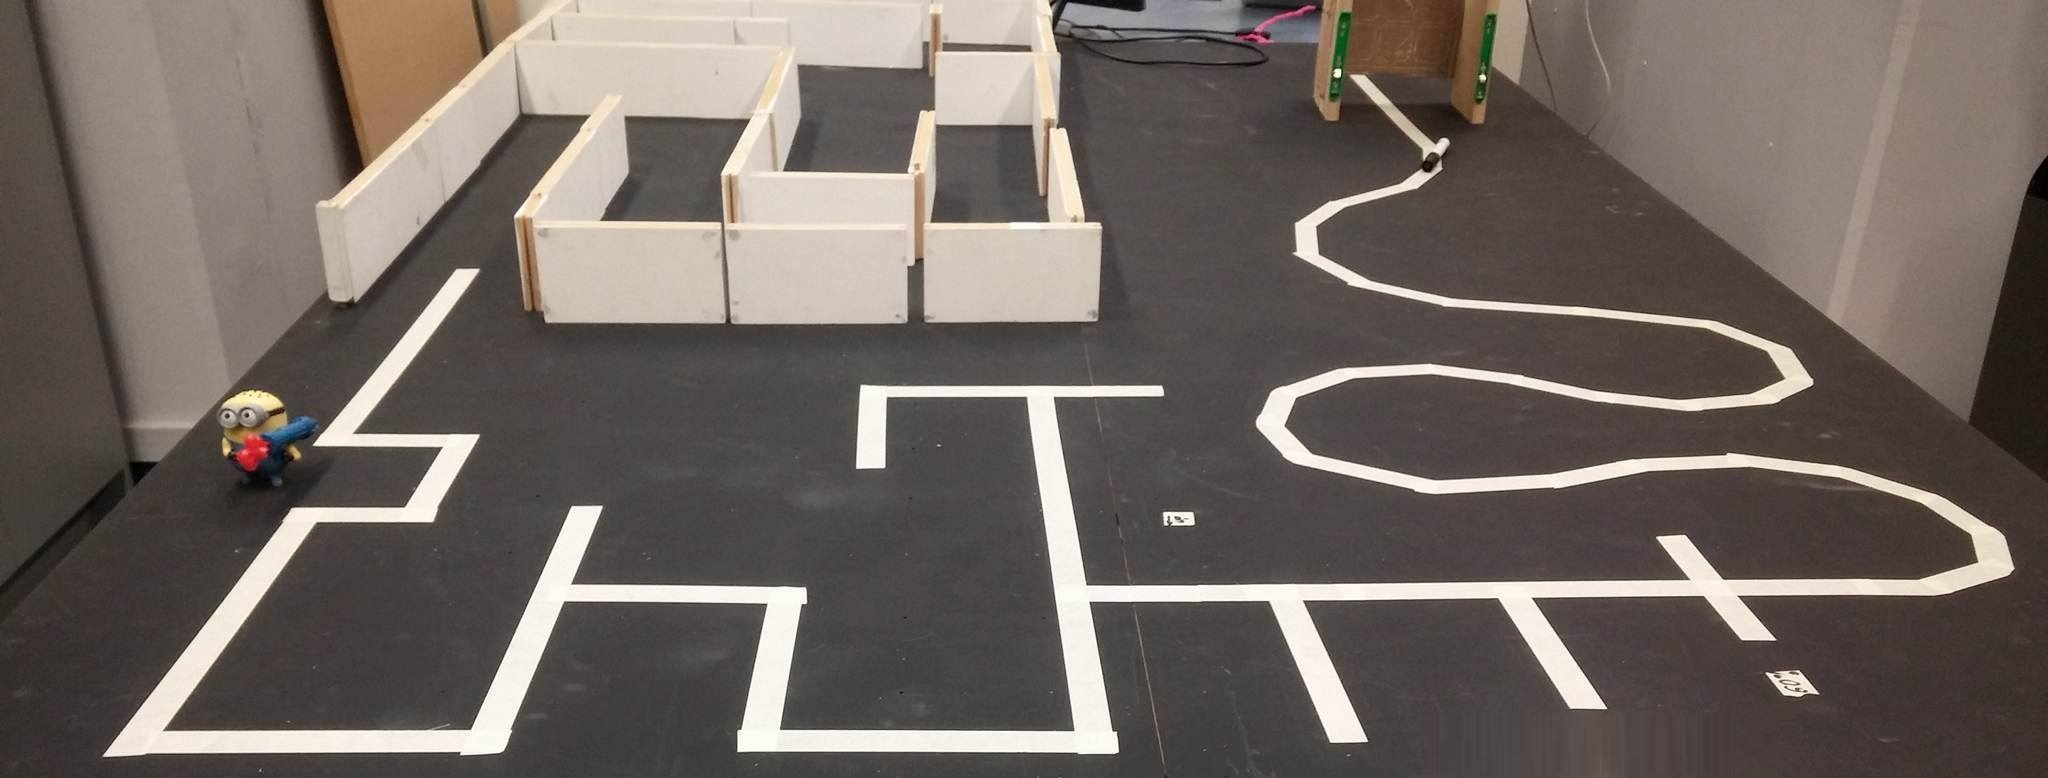
\includegraphics[width=\textwidth]{maze}
  \centering
  \caption{The Maze used to test the Autonomous vehicle}
\end{figure}
\subsection{Interpretation}
\subsection{Discussion}
The decision to not have a rear wheel, was made because it would give a greater
ability to turn the vehicle and make the AVC more responsive to the change in
environment.\\
The co-efficient of proportionality is much higher then derivative which is
higher than the integral response, to better respond to the present situation.\\
The Camera appears to be broken on further expectation right now, so we can't show
any results\\
The networking section, works flawlessly at the present, and causes the bridge
to raise and lower as required.
\section{Conclusion}
\subsection{Assessment}
\subsection{Recommendations}
\section{Bibliography}
\printbibliography{}
\section{Appendix}
\subsection{Weekly Log}
\subsubsection*{Week 1}
\begin{tabularx}{\textwidth}{clX}
  \scalecheck & ALL      & Construct a Project Plan and Contact Julius\\
  \scalecheck & Rhaz     & Organise Meeting\\
  \scalecheck & Jacob    & Create GitHub and Establish Facebook Chat\\
  \scalecheck & Andrew   & Study SSH for Thursday Meeting\\
  \scalecheck & Mitchell & Study Unit Testing\\
  \scalecheck & Theo     & Make a general plan for the chassis\\
  \scalecheck & Julius   & Get in contact with the group
\end{tabularx}
\subsubsection*{Week 2}
\begin{tabularx}{\textwidth}{clX}
  \scalecheck  & ALL      & Discuss ideas and start on the AVC Code\\
  \scalecheck  & Rhaz     & Keep up to date on weekly tasks\\
               & Jacob    & Robot moving in straight line --- appears to work, but haven't tested with a battery yet\\
  \scalecheck  & Andrew   & Complete the README.md\\
  \scalecheck  & Mitchell & Look into the networking code, and how it works\\
  \scalecheck  & Theo     & Figure out how to use the CAD software\\
               & Julius   & Show Up --- Not turned up --- Postponed\\
\end{tabularx}
\subsubsection*{Week 3}
\begin{tabularx}{\textwidth}{clX}
  \scalecheck & ALL      & Progress update with team members and begin writing progress report\\
  \scalecheck & Rhaz     & Robot Opens Gate\\
  \scalecheck & Jacob    & Robot Opens Gate\\
  \scalecheck & Andrew   & Robot Opens Gate\\
  \scalecheck & Mitchell & Update the README create Hardware updates and assist in the hardware efforts.\\
  \scalecheck & Theo     & Create a non-powered wheel case and battery case for the robot\\
              & Julius   & Show up and contribute to team meetings\\
\end{tabularx}
\subsubsection*{Week 4}
\begin{tabularx}{\textwidth}{clX}
  \scalecheck & ALL      & Progress update with team members\\
  \scalecheck & Rhaz     & Quadrant 1 completed\\
  \scalecheck & Jacob    & Quadrant 1 completed\\
  \scalecheck & Andrew   & Quadrant 1 completed\\
  \scalecheck & Mitchell & Assist in hardware and pre-reading for quadrant 2\\
              & Theo     & Attach sensors to robot so it can detect the maze and obstructions --- postponed as code not up to that section yet.\\
              & Julius   & Contribute in some way\\
\end{tabularx}
\subsubsection*{Week 5}
\begin{tabularx}{\textwidth}{clX}
  \scalecheck & ALL      & Progress update with team members\\
  \scalecheck & Rhaz     & PID system functioning\\
  \scalecheck & Jacob    & PID system functioning\\
  \scalecheck & Andrew   & PID system functioning\\
  \scalecheck & Mitchell & Bug fixing and tinker with PID constants\\
  \scalecheck & Theo     & Make battery clip easier\\
              & Julius   & Contribute in some way\\
\end{tabularx}
\subsubsection*{Week 6}
\begin{tabularx}{\textwidth}{clX}
              & ALL      & Quadrant 3 complete\\
              & Rhaz     & Quadrant 3 complete\\
              & Jacob    & Quadrant 3 complete\\ 
              & Andrew   & Quadrant 3 complete\\ 
              & Mitchell & Quadrant 3 complete\\ 
  \scalecheck & Theo     & Attaching sensors to navigate Quadrant 4\\
              & Julius   & Contribute in some way\\
\end{tabularx}
\end{document}
